\section{Software and Documentation}

\begin{itemize}
\item All software that developed for this thesis is available and will be maintained at \textbf{\url{https://github.com/karadalex/surgery_robotics_kuka_barrett}}
\item Instruction on how to run the software of this thesis, as well as documentation of the various software components is available and will be maintained at 
	\textbf{\url{https://karadalex.github.io/surgery_robotics_kuka_barrett/}}
\end{itemize}

\begin{center}
\begin{figure}[!htb]
\centering
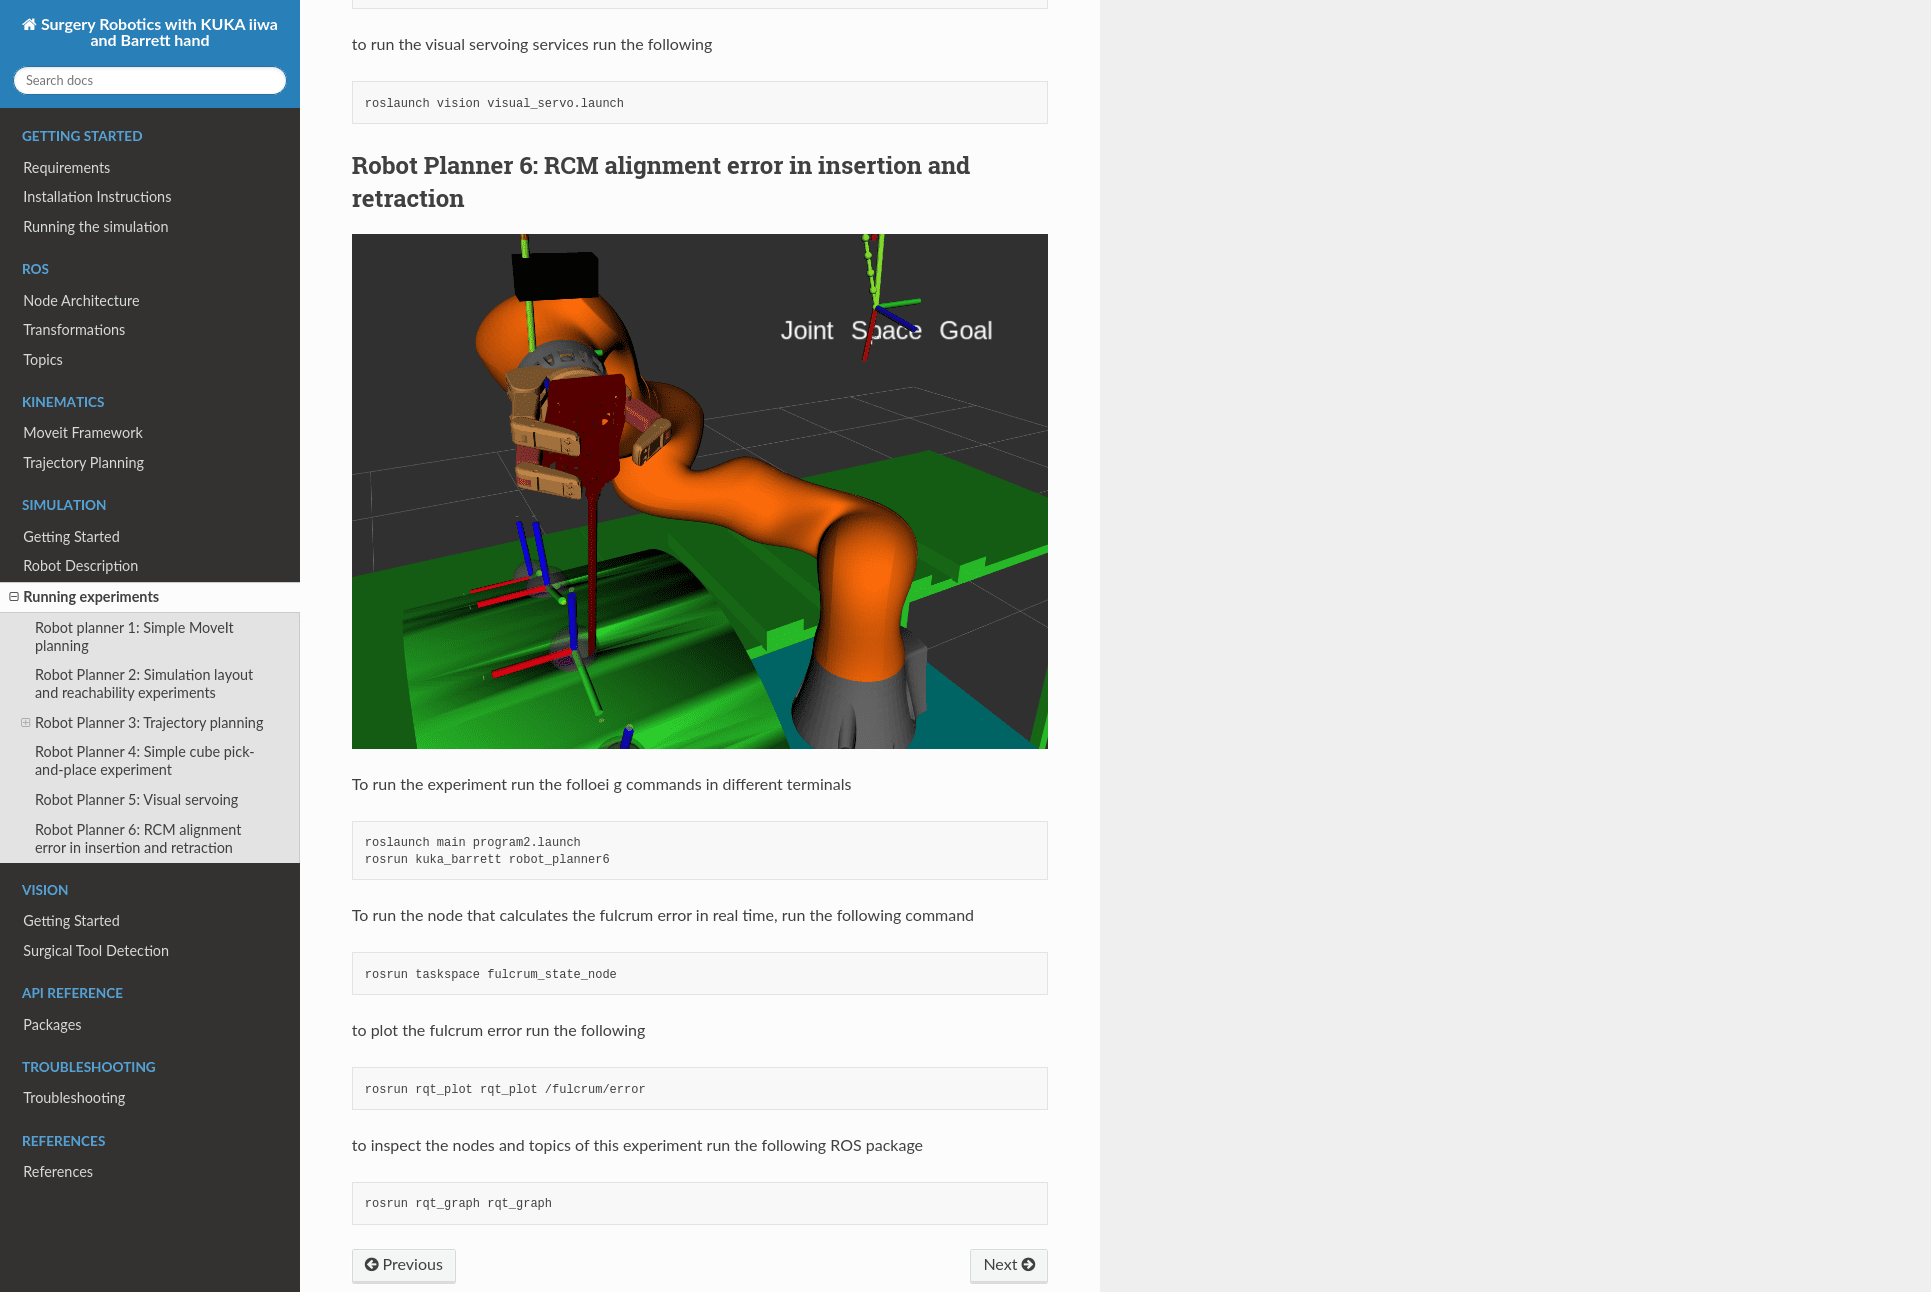
\includegraphics[width=\textwidth]{images/documentation.png}
\caption{Documentation written with Sphinx and rosdoc\_lite }
\label{documentation}
\end{figure}
\end{center}

\section{Mathematics}

\subsection{Euler angles to Quaternions}

Let $\theta, \phi, \psi$ be the Euler angles (roll, pitch, yaw) respectively, then using the following equations
\[
cθ = cos\left( \frac{θ}{2} \right) , sθ = sin\left( \frac{θ}{2} \right)
\]
\[
cφ = cos\left( \frac{φ}{2} \right) , sφ = sin\left( \frac{φ}{2} \right)
\]
\[
cψ = cos\left( \frac{ψ}{2} \right) , sψ = sin\left( \frac{ψ}{2} \right)
\]

we can calculate the associated quaternion, in vector notation, as follows

\[
\mathbf{q} = \begin{bmatrix} q_x \\ q_y \\ q_z \\ q_w \end{bmatrix} = \begin{bmatrix}
sθcφcψ - cθsφsψ \\
cθsφcψ + sθcφsψ \\
cθcφsψ - sθsφcψ \\
cθcφcψ + sθsφsψ \\
\end{bmatrix}
\]

\subsection{Cartesian to spherical coordinates}

\[
r = \sqrt{x^2+y^2+z^2}
\]

\[
θ = atan2(\sqrt{x^2 + y^2}, z)
\]

\[
φ = atan2(y, x)
\]


\subsection{Spherical to cartesian coordinates}

\[
x = rsin(θ)cos(φ)
\]

\[
y = rsin(θ)sin(φ)
\]

\[
z = rcos(θ)
\]

